\documentclass{article}

\usepackage[bookmarksnumbered, colorlinks, plainpages]{hyperref}
\usepackage{fancyhdr}
\usepackage{extramarks}
\usepackage{amsmath}
\usepackage{amsthm}
\usepackage{amsfonts}
\usepackage{tikz}
\usepackage[plain]{algorithm}
\usepackage{algpseudocode}
\usepackage{graphicx}
\usepackage{tabularx}

\graphicspath{ {./img/} }
\usetikzlibrary{automata, positioning}

%
% Basic Document Settings
%

\topmargin=-0.45in
\evensidemargin=0in
\oddsidemargin=0in
\textwidth=6.5in
\textheight=9.0in
\headsep=0.25in

\linespread{1.1}

\pagestyle{fancy}
\lhead{\hmwkAuthorName}
\chead{\hmwkClass\ (\hmwkClassInstructor\ \hmwkClassTime): \hmwkTitle}
\rhead{\firstxmark}
\lfoot{\lastxmark}
\cfoot{\thepage}

\renewcommand\headrulewidth{0.4pt}
\renewcommand\footrulewidth{0.4pt}

\setlength\parindent{0pt}

%
% Create Problem Sections
%

\newcommand{\enterProblemHeader}[1]{
    \nobreak\extramarks{}{Problem \arabic{#1} continued on next page\ldots}\nobreak{}
    \nobreak\extramarks{Problem \arabic{#1} (continued)}{Problem \arabic{#1}
    continued on next page\ldots}\nobreak{}
}

\newcommand{\exitProblemHeader}[1]{
    \nobreak\extramarks{Problem \arabic{#1} (continued)}{Problem \arabic{#1}
    continued on next page\ldots}\nobreak{}
    \stepcounter{#1}
    \nobreak\extramarks{Problem \arabic{#1}}{}\nobreak{}
}

\setcounter{secnumdepth}{0}
\newcounter{partCounter}
\newcounter{homeworkProblemCounter}
\setcounter{homeworkProblemCounter}{1}
\nobreak\extramarks{Problem \arabic{homeworkProblemCounter}}{}\nobreak{}

%
% Homework Problem Environment
%

\newenvironment{homeworkProblem}[1]{
    \section{Problem \arabic{homeworkProblemCounter}{#1}}
    \setcounter{partCounter}{1}
    \enterProblemHeader{homeworkProblemCounter}
}{
    \exitProblemHeader{homeworkProblemCounter}
}

%
% Homework Details
%   - Title
%   - Due date
%   - Class
%   - Section/Time
%   - Instructor
%   - Author
%

\newcommand{\hmwkTitle}{Homework\ 5}
\newcommand{\hmwkDueDate}{April 25, 2024}
\newcommand{\hmwkClass}{CS 401}
\newcommand{\hmwkClassTime}{9:30am}
\newcommand{\hmwkClassInstructor}{Professor Sidiropoulos}
\newcommand{\hmwkAuthorName}{\textbf{Ryan Magdaleno}}
\newcommand{\hwline}{\begin{center}\line(1,0){358px}\end{center}}

%
% Title Page
%

\title{
    \vspace{2in}
    \textmd{\textbf{\hmwkClass:\ \hmwkTitle}}\\
    \normalsize\vspace{0.1in}\small{Due\ on\ \hmwkDueDate\ at 11:59pm}\\
    \vspace{0.1in}\large{\textit{\hmwkClassInstructor\ \hmwkClassTime}}
    \vspace{3in}
}

\author{\hmwkAuthorName\\\href{mailto:rmagd2@uic.edu}{rmagd2@uic.edu}}
\date{}

\renewcommand{\part}[1]{\textbf{\large Part \Alph{partCounter}}
\stepcounter{partCounter}\\}
%
% Various Helper Commands
%

% Useful for algorithms
\newcommand{\alg}[1]{\textsc{\bfseries \footnotesize #1}}

% For derivatives
\newcommand{\deriv}[1]{\frac{\mathrm{d}}{\mathrm{d}x} (#1)}

% For partial derivatives
\newcommand{\pderiv}[2]{\frac{\partial}{\partial #1} (#2)}

% Integral ds
\newcommand{\dx}{\mathrm{d}x}
\newcommand{\D}[1]{\mathrm{d}#1}

% Image insertion
\newcommand{\img}[2]{\begin{center}\includegraphics[scale=#1]{#2}\end{center}}

% Alias for the Solution section header
\newcommand{\solution}{\textbf{\large Solution}\\}

% Probability commands: Expectation, Variance, Covariance, Bias
\newcommand{\E}{\mathrm{E}}
\newcommand{\Var}{\mathrm{Var}}
\newcommand{\Cov}{\mathrm{Cov}}
\newcommand{\Bias}{\mathrm{Bias}}

\begin{document}

\maketitle

\pagebreak

%%%%%%%%%%%%%%%%%%%%%%%%%%%%%%%%%%%%%%%%%%%%%%%%%%%%%%%%%%%%%%%%%%%%%%%%%%%%%%%%%%%%%%%%%

\begin{homeworkProblem}{: Evacuating a building.}
    \hspace{10pt}
    In an emergency, a building has to be evacuated in a hurry. When a disaster strikes
    an evacuation plan should be in place and there are many aspects that such a plan 
    takes into consideration: \href{https://www.osha.gov/SLTC/etools/evacuation/evac.html}
    {https://www.osha.gov/SLTC/etools/evacuation/evac.html.} Let us consider a much 
    simplified version. Let $G = (V, E)$ be a directed graph, representing a building. 
    Every vertex $v\in V$ represents a room, and every edge $(u, v)\in E$ represents a 
    corridor that leads from room $u$ to room $v$ (there may be also an edge $(v, u)$). 
    For every corridor $(u, v)\in E$, at most $c_{u,v}$ people can traverse it 
    simultaneously in the direction from $u$ to $v$, where $c_{u,v}$ is a positive 
    integer. Traversing a corridor takes one time step, and traversing a room takes zero 
    time.

    \vspace{10pt}\hspace{10pt}
    Suppose that there are $k$ people in the building, all initially located in some room 
    $s\in V$, and they all want to move to some room $t\in V$ (e.g., exit). Give an 
    algorithm that computes the fastest possible way for all people to move from room $s$ 
    to room $t$. The running time of your algorithm should be polynomial in both $n$, and 
    $k$ (for example, $O\left(\left|V\right|^{10}k^{10}\right)$.

    \vspace{10pt}\hspace{10pt}
    \textit{Hint}: Clearly, this problem seems related to the max-flow problem. However, 
    an additional complication in building evacuation is that the algorithm has to 
    account for time. One possible approach for overcoming this obstacle is as follows: 
    First, argue that the maximum time necessary to evacuate the building it at most 
    $O(kn)$ (why?). It is enough to solve the following simpler “decision” version of the 
    problem: Given some integer $T$ , find a way to evacuate the building in at most $T$ 
    steps, if possible. Given an algorithm for the decision problem we can solve the 
    original problem by trying all $O(kn)$ possible values for $T$. Finally, show that 
    the decision problem can be reduced to a max-flow computation; that is, construct a 
    flow network $N_T$, such that the building can be evacuated in at most $T$ steps, if 
    and only if the max-flow in $N_T$ has value at least $k$.

    \hwline\solution
    \vspace{-28pt}\subsection{kn time complexity}
    The reason the time to evacuate the building is $O(kn)$ is that for each person in 
    the building ($k$), we need to find room $t$ which in the worst case would require us 
    to traverse $n$ rooms, therefore for everyone to exit the building, the time 
    complexity is $O(kn)$.
    \hwline
    \vspace{-20pt}\subsection{High Level Algorithm Explanation}
    \begin{enumerate}
        \item\vspace{-5pt}
        Create a flow network $N$ with $n$ vertices representing the rooms, and edges
        representing each corridor ($u,v$) with capacity $c_{u,v}$.
        \item\vspace{-5pt}
        Connect a source node $A$ to the starting room $s$ with an edge capacity of $k$.
        \item\vspace{-5pt}
        Connct a sink node $Z$ to the exit room $t$ with an edge capacity of $\infty$.
        \item\vspace{-5pt}
        Construct a flow network $N_T$ based on our building graph and some given $T$ 
        time constraint, check all values ranging from $T=1$ to $T=kn$ until $N_T$'s max 
        flow is at least $k$, this minimum $T$ value is the shortest amount of time. This 
        can be sped up with binary search rather than a linear check. Adjust the 
        capacities of the edges to account for time, for edges between rooms, if $T$ is 
        $<$ than the $c_{u,v}$ of that room, set it to $T$, else keep $c_{u, v}$, this 
        prevents the flow from exceeding the time constraint.
    \end{enumerate}
    \hwline\pagebreak

    \subsection{Time Complexity Justification}
    \hspace{10pt}Constructing the flow network requires checking each corridor, resulting 
    in $O(n^2)$, where $n$ is the number of vertices/rooms in the graph.

    \vspace{10pt}\hspace{10pt}The binary search to find the $T$ value takes $O(\log(kn))$.

    \vspace{10pt}\hspace{10pt}The capacity adjustments and maximum flow calculations is 
    done against each binary search, the capacity adjustments take $O(n^2)$ time due to 
    us modifying/checking each corridor. Computing the maximum flow using 
    Ford-Fulkerson's algorithm takes $O(maxflow\cdot n^2)$ where $n^2$ is the number of 
    edges in the graph, the maxflow can be at most $k$ so we get $O(n^2 \cdot k)$.

    \vspace{10pt}Putting everything together we get the following time complexity:
    \begin{align*}
        T(n, k) &= O(n^2 + \log(kn)\cdot n^2 \cdot k) \\
        T(n, k) &= \boxed{O(\log(kn)\cdot n^2 \cdot k)}
    \end{align*}
    where $n$ is the number of rooms and $k$ is the number of people.
    \hwline\pagebreak
\end{homeworkProblem}
\pagebreak

%%%%%%%%%%%%%%%%%%%%%%%%%%%%%%%%%%%%%%%%%%%%%%%%%%%%%%%%%%%%%%%%%%%%%%%%%%%%%%%%%%%%%%%%%

\begin{homeworkProblem}{: Paper reviewing.}
    \hspace{10pt}
    Computer science is “the only scientific community that considers conference 
    publication as the primary means of publishing our research results” (rather than 
    journals): \href{https://cacm.acm.org/opinion/conferences-vs-journals-in-computing-research/}{https://cacm.acm.org/opinion/conferences-vs-journals-in-computing-research/}. In other disciplines, a 
    “publication” means a paper has appeared in what is known a “refereed” and indexed 
    (by an officially recognized body, such as the Web of Science) journal. So in 
    computer science, the conference publications are reviewed (by volunteer researchers, 
    such as your professors, for the so-called honor of having a line in your resume that 
    says they served as a member of the conference Program Committee). Suppose a 
    conference receives $n$ paper submissions and there are $m$ members of the Program 
    Committee. The Program Committee members then bid on which papers they can and are 
    willing to review. After that, reviewers are assigned to papers (from among those 
    they bid on) so that each paper has, lets say, at least 3 reviewers and each     
    reviewer reviews at most, lets say, 5 papers. (The reviewers collective scores then 
    decide whether a paper is accepted for the conference or not. Typically, for a good 
    conference, only about 20\% of the papers are accepted.)

    \vspace{10pt}\hspace{10pt}
    Design and analyze a polynomial-time algorithm to make the assignment of reviewers to 
    papers (so that each reviewer reviews only the papers they bid on and the min and max 
    constraints are respected) or decide that no feasible assignment exists.

    \hwline\solution
    \vspace{-28pt}\subsection{High Level Algorithm Explanation}
    \begin{enumerate}
        \item\vspace{-5pt}
        We need to construct a directed bipartite graph flow network as follows:
        \vspace{-5pt}\begin{enumerate}
            \item\vspace{-5pt}
            We create nodes representing the reviewers $R_1$ to $R_m$.
            \item\vspace{-5pt}
            We create nodes representing the papers $P_1$ to $P_n$.
            \item\vspace{-5pt}
            A source node $s$ and a sink node $t$.
            \item\vspace{-5pt}
            We shall assign capacities from the source node $s$ to each reviewer, each 
            reviewer can review at most 5 papers, so a capacity of 5 is needed.
            \item\vspace{-5pt}
            We shall assign capacities from each reviewer to each of their desired 
            papers, a capacity of 1 is needed because that reviewer can review that paper 
            only once.
            \item\vspace{-5pt}
            We shall assign capacities from each paper to the sink node $t$, each paper 
            will have a capacity of 3 representing the minimum reviewers needed for that 
            paper.
        \end{enumerate}
        \item\vspace{-5pt}
        We can now use Ford-Fulkerson's algorithm to find the maximum flow in our newly 
        constructed network.
        \item\vspace{-5pt}
        We must ensure that each paper has at least 3 reviewers and each reviewer has at 
        most 5 papers assigned, we shall do the following to check this:
        \vspace{-5pt}\begin{enumerate}
            \item\vspace{-5pt}
            For each paper node $P_1$ to $P_n$, sum up the flow coming into it. This 
            represents the number of reviewers assigned to the current paper, if the flow 
            sum is $<3$ then reject, else continue.
            \item\vspace{-5pt}
            For each reviewer node $R_1$ to $R_m$, sum up the outgoing flow, each 
            outgoing edge representing a desired paper, the total flow is the number 
            papers assigned, if the flow for the current reviewer node is $>5$ then 
            reject, else accept.
        \end{enumerate}
        \vspace{-10pt}\hwline\pagebreak
        Here's an example of my proposed flow network.
        \begin{center}
            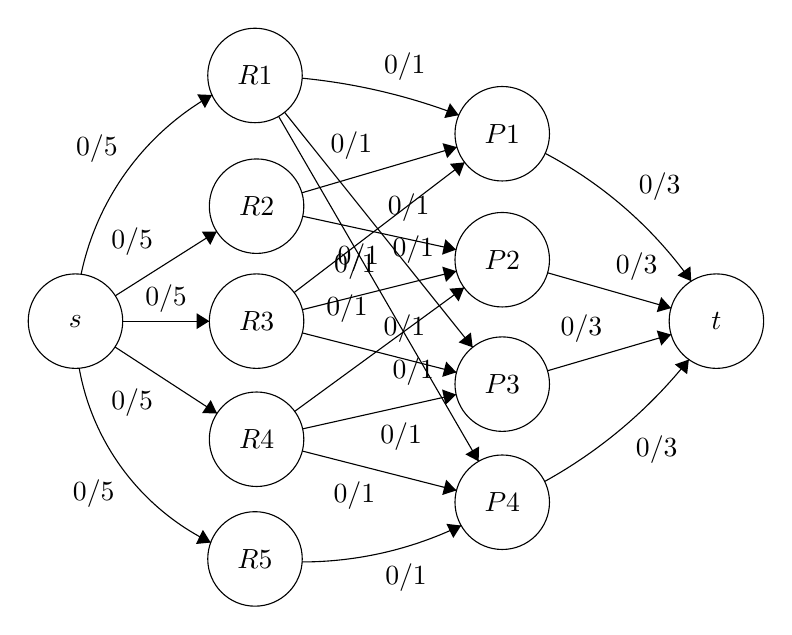
\begin{tikzpicture}[scale=0.2]
            \tikzstyle{every node}+=[inner sep=0pt]
            \draw [black] (15.8,-26.2) circle (3);
            \draw (15.8,-26.2) node {$s$};
            \draw [black] (27.3,-18.9) circle (3);
            \draw (27.3,-18.9) node {$R2$};
            \draw [black] (27.3,-26.2) circle (3);
            \draw (27.3,-26.2) node {$R3$};
            \draw [black] (27.3,-33.7) circle (3);
            \draw (27.3,-33.7) node {$R4$};
            \draw [black] (42.9,-14.3) circle (3);
            \draw (42.9,-14.3) node {$P1$};
            \draw [black] (42.9,-22.3) circle (3);
            \draw (42.9,-22.3) node {$P2$};
            \draw [black] (42.9,-30.2) circle (3);
            \draw (42.9,-30.2) node {$P3$};
            \draw [black] (42.9,-37.7) circle (3);
            \draw (42.9,-37.7) node {$P4$};
            \draw [black] (56.5,-26.2) circle (3);
            \draw (56.5,-26.2) node {$t$};
            \draw [black] (27.2,-10.6) circle (3);
            \draw (27.2,-10.6) node {$R1$};
            \draw [black] (27.2,-41.3) circle (3);
            \draw (27.2,-41.3) node {$R5$};
            \draw [black] (18.33,-24.59) -- (24.77,-20.51);
            \fill [black] (24.77,-20.51) -- (23.82,-20.51) -- (24.36,-21.36);
            \draw (19.4,-22.05) node [above] {$0/5$};
            \draw [black] (18.8,-26.2) -- (24.3,-26.2);
            \fill [black] (24.3,-26.2) -- (23.5,-25.7) -- (23.5,-26.7);
            \draw (21.55,-25.7) node [above] {$0/5$};
            \draw [black] (18.31,-27.84) -- (24.79,-32.06);
            \fill [black] (24.79,-32.06) -- (24.39,-31.21) -- (23.84,-32.04);
            \draw (19.4,-30.45) node [below] {$0/5$};
            \draw [black] (30.18,-18.05) -- (40.02,-15.15);
            \fill [black] (40.02,-15.15) -- (39.11,-14.9) -- (39.4,-15.85);
            \draw (33.32,-15.99) node [above] {$0/1$};
            \draw [black] (30.23,-19.54) -- (39.97,-21.66);
            \fill [black] (39.97,-21.66) -- (39.29,-21) -- (39.08,-21.98);
            \draw (33.76,-21.28) node [below] {$0/1$};
            \draw [black] (30.21,-25.47) -- (39.99,-23.03);
            \fill [black] (39.99,-23.03) -- (39.09,-22.74) -- (39.33,-23.71);
            \draw (33.55,-23.6) node [above] {$0/1$};
            \draw [black] (30.23,-33.04) -- (39.97,-30.86);
            \fill [black] (39.97,-30.86) -- (39.08,-30.54) -- (39.3,-31.52);
            \draw (36.48,-32.62) node [below] {$0/1$};
            \draw [black] (30.21,-34.45) -- (39.99,-36.95);
            \fill [black] (39.99,-36.95) -- (39.34,-36.27) -- (39.09,-37.24);
            \draw (33.51,-36.34) node [below] {$0/1$};
            \draw [black] (30.21,-26.95) -- (39.99,-29.45);
            \fill [black] (39.99,-29.45) -- (39.34,-28.77) -- (39.09,-29.74);
            \draw (36.69,-27.56) node [above] {$0/1$};
            \draw [black] (16.157,-23.225) arc (168.1471:119.53653:17.125);
            \fill [black] (24.47,-11.84) -- (23.53,-11.8) -- (24.02,-12.67);
            \draw (18.51,-15.25) node [left] {$0/5$};
            \draw [black] (24.393,-40.255) arc (-116.0299:-169.8669:15.318);
            \fill [black] (24.39,-40.26) -- (23.89,-39.45) -- (23.45,-40.35);
            \draw (18.31,-37.12) node [left] {$0/5$};
            \draw [black] (30.194,-10.773) arc (84.43897:69.03931:38.146);
            \fill [black] (40.14,-13.12) -- (39.58,-12.36) -- (39.22,-13.3);
            \draw (36.71,-10.95) node [above] {$0/1$};
            \draw [black] (29.08,-12.94) -- (41.02,-27.86);
            \fill [black] (41.02,-27.86) -- (40.91,-26.92) -- (40.13,-27.55);
            \draw (35.61,-18.98) node [right] {$0/1$};
            \draw [black] (29.69,-24.38) -- (40.51,-16.12);
            \fill [black] (40.51,-16.12) -- (39.58,-16.21) -- (40.18,-17);
            \draw (37.25,-20.75) node [below] {$0/1$};
            \draw [black] (29.72,-31.93) -- (40.48,-24.07);
            \fill [black] (40.48,-24.07) -- (39.54,-24.14) -- (40.13,-24.95);
            \draw (37.25,-28.5) node [below] {$0/1$};
            \draw [black] (28.7,-13.2) -- (41.4,-35.1);
            \fill [black] (41.4,-35.1) -- (41.43,-34.16) -- (40.56,-34.66);
            \draw (34.4,-25.39) node [left] {$0/1$};
            \draw [black] (40.29,-39.175) arc (-64.21614:-89.9546:23.258);
            \fill [black] (40.29,-39.18) -- (39.35,-39.07) -- (39.79,-39.97);
            \draw (36.79,-41.57) node [below] {$0/1$};
            \draw [black] (54.751,-28.636) arc (-38.48063:-61.08444:30.6);
            \fill [black] (54.75,-28.64) -- (53.86,-28.95) -- (54.64,-29.57);
            \draw (52.71,-33.45) node [below] {$0/3$};
            \draw [black] (45.78,-29.35) -- (53.62,-27.05);
            \fill [black] (53.62,-27.05) -- (52.71,-26.79) -- (53,-27.75);
            \draw (47.93,-27.59) node [above] {$0/3$};
            \draw [black] (45.78,-23.13) -- (53.62,-25.37);
            \fill [black] (53.62,-25.37) -- (52.99,-24.67) -- (52.71,-25.63);
            \draw (51.44,-23.63) node [above] {$0/3$};
            \draw [black] (45.627,-15.546) arc (62.20642:35.42173:26.606);
            \fill [black] (54.9,-23.66) -- (54.85,-22.72) -- (54.03,-23.3);
            \draw (52.9,-18.57) node [above] {$0/3$};
            \end{tikzpicture}
        \end{center}
    \end{enumerate}
    \hwline
    \vspace{-24pt}\subsection{Time Complexity Justification}
    \hspace{10pt}Creating the flow network graph involves iterating over all papers and
    reviewers to create capacity 1 edges, this takes $O(n\cdot m)$ time.

    \vspace{10pt}\hspace{10pt}Adding the source and sink capacity connections can be done 
    during the previous step on each node giving a $O(n\cdot m)$ time complexity.

    \vspace{10pt}\hspace{10pt}Computing the maximum flow using Ford-Fulkerson's algorithm 
    takes $O(maxflow\cdot (nm + n + m))$, note the $nm + n + m$ term represents the total 
    edges in the graph. $nm=$ reviewers to papers, $n=$ papers to sink, and $m=$ source 
    to reviewer connections. This is determined by the number of augmenting paths needed 
    to reach the maximum flow.

    \vspace{10pt}All together our combined time complexity is as follows:
    \begin{align*}
        T(n, m, maxflow) &= \boxed{O(n m + maxflow\cdot (nm + n + m))}
    \end{align*}
    where $n$ is the number of papers and $m$ is the number of researchers.
    \hwline
\end{homeworkProblem}

%%%%%%%%%%%%%%%%%%%%%%%%%%%%%%%%%%%%%%%%%%%%%%%%%%%%%%%%%%%%%%%%%%%%%%%%%%%%%%%%%%%%%%%%%

\end{document}